In this section we describe our experiments and comment the results we got. For brevity's sake, if not otherwise specified, we will refer to CFM with target level (algorithm \ref{alg:CFM-TL}]) simply as CFM. 

\subsection{Methodological note}
The objective function defined in \ref{obj_fun} is not theoretically ensured to converge, as we extensively explained in section \ref{convergence}. Still, this is not a big issue when training a MLP model. In fact, the global convergence of the training loss is not even desired at all, as it may imply the overfitting of the training data, worsening the generalization capabilities of the model. Thus, it is very common in machine learning to apply an optimization algorithm even without theoretical guarantees, and settle for non optimal solutions.

\subsection{Dataset and general settings}
The dataset we used for our experiments is the ML-CUP21 dataset, from the \textit{Machine Learning CUP 2021-2022} student competition of the Machine Learning course at University of Pisa. This dataset consists of 1477 samples, each of which is defined by 10 numerical input features and 2 numerical targets.

Unless otherwise specified, whenever we trained a model, we set a maximum number of epochs of 10000. As a further stopping criterion, we allowed for early stopping, with a tolerance of $10^{-4}$ and a patience of 150 epochs, to prevent trainings to zigzag too much between suboptimal solutions.

We also made large use of grid search, and tested the hyperparameters combinations with different random initializations of the weights of the models, to get some understanding of the variances of the optimization algorithms presented. In both these situations, the random seeds for the weights inizialization were the same. This was done to guarantee the same starting points when training a model with different algorithms, thus avoiding introducing biases based on more or less lucky initializations.

When training a model with CFM, we limited ourselves to consider the thresholds $\delta^{(i)} = \frac{a}{a+i}$, with $a \in \R$.
Note that this set of sequences verifies the hypothesis outlined in \ref{cfm_conv}. Of course, this does not imply theoretical convergence by itself; still, we wanted our hyperparameter choice to be as close as possible to the theoretical requirements for convergence.

Lastly, table \ref{tab:epoch_times} shows the average time per epoch for each of the experiments done. As we can see, there is no relevant difference between the time required by HBG and CFM to complete an epoch of training. For this reason, for the sake of simplicity, we limited ourselves to the number of epochs as the only metric of comparison between the speed of the two algorithms.

\begin{table}[htbp]
    \begin{adjustwidth}{-2cm}{-2cm}
        \centering
        \begin{tabular}{|c|c|c|}
            \hline
            Experiment 0.2 & \multicolumn{2}{|c|}{\makecell{HBG: $2.719 \pm 0.068$ \\ CFM with target level: $2.845 \pm 0.022$ \\ CFM with exact Polyak step size: $2.796 \pm 0.073$}} \\
            \hline
            \multirow{2}{*}[-1ex]{Experiment 1} & Sigmoid & \makecell{HBG: $8.221 \pm 0.123$ \\ CFM: $8.975 \pm 0.187$} \\
            \cline{2-3}
            & ReLU & \makecell{HBG: $3.476 \pm 0.153$ \\ CFM: $3.408 \pm 0.094$} \\
            \hline
            \multirow{2}{*}[-1ex]{Experiment 2} & Sigmoid & \makecell{HBG: $10.864 \pm 0.554$ \\ CFM: $10.553 \pm 0.106$} \\
            \cline{2-3}
            & ReLU & \makecell{HBG: $4.853 \pm 0.066$ \\ CFM with target level: $5.131 \pm 0.070$ \\ CFM with exact Polyak step size: $4.991 \pm 0.084$} \\
            \hline
            Experiment 3 & \multicolumn{2}{|c|}{\makecell{HBG: $7.781 \pm 0.283$ \\ CFM: $7.990 \pm 0.079$}} \\
            \hline
        \end{tabular}
    \end{adjustwidth}
    \caption{Average time per epoch (ms)}
    \label{tab:epoch_times}
\end{table}

\subsection{Experiment 0.1 - Threshold influence in CFM}
\label{exp01}
In the first preliminary experiment we wanted to test the influence of the target level threshold on CFM speed of convergence and accuracy. To do so, we set up a network with a 30 neurons hidden layer, ReLU activation function and L1 regularization with $\lambda = 0.1$, and we trained 5 different models with CFM, with $a \in \{50,75,100,150,200\}$ and $\gamma = 0.5$. The results are shown in figure \ref{fig:threshold}.

\begin{figure}[htbp]
    \begin{subfigure}{.5\textwidth}
        \centering
        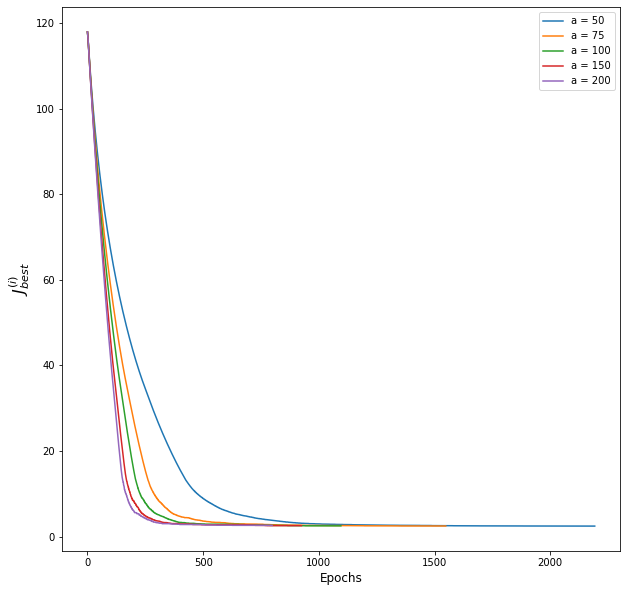
\includegraphics[width=.9\textwidth]{images/threshold_convergence_speed.png}
        \label{fig:speed_acc}
    \end{subfigure}%
    \begin{subfigure}{.5\textwidth}
        \centering
        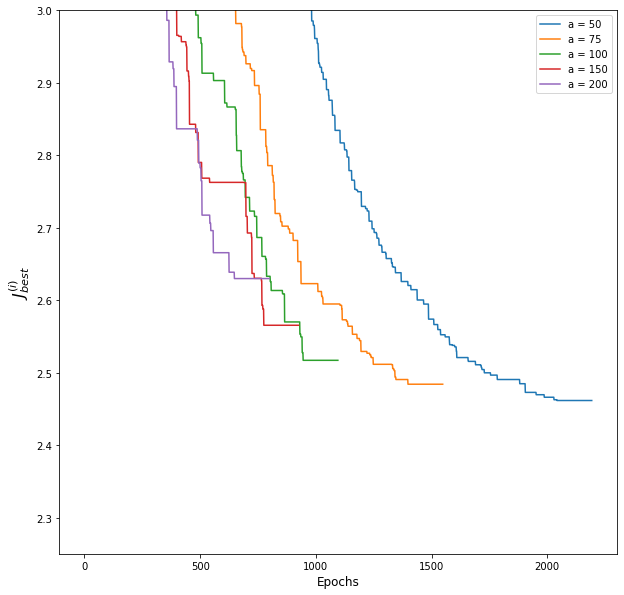
\includegraphics[width=.9\textwidth]{images/threshold_convergence_speed_zoom.png}
        \label{fig:speed_acc_zoom}
    \end{subfigure}
    \caption{Threshold influence in CFM}
    \label{fig:threshold}
\end{figure}

As we can see, larger values of $a$ lead to a faster convergence, but to a worse result, thus defining a very sharp trade-off between the speed of convergence of the algorithm and the suboptimality of the solution found (cfr. \ref{bibitem:boyd}). In light of this result, when performing grid search for CFM in the following experiments, we kept fixed the threshold value to guarantee a reasonable trade-off between speed and accuracy of convergence, and we fine tuned only the momentum hyperparameter.

\subsection{Experiment 0.2 - Convex loss function}
\label{exp02}
In the second preliminary experiment we wanted to test the presented algorithms on a convex function. Thus, to enforce the convexity of the loss, we built a MLP with identity as activation function. Of course, such a network serves no practical purpose, but lets us show the results presented in \ref{convergence}.

Specifically, we built a MLP with a single hidden layer composed by 60 neurons. The Lasso regularization coefficient was set to $\lambda = 0.1$. We fine tuned the hyperparameters via a grid search, as shown in table \ref{tab:02_gs}.

\begin{table}[htbp]
    \centering
    \begin{tabular}{|c|c|}
        \hline
        HBG & \makecell{$\alpha \in 10^{-3} \times \{0.5, 0.75, 1, 2.5, 5, 7.75, 10, 25, 50\}$ \\ $\beta \in \{0.1, 0.25, 0.5, 0.75, 0.9\}$} \\
        \hline
        CFM & \makecell{$\gamma \in \{0.1, 0.15, 0.2, 0.3, 0.4, 0.5, 0.6, 0.75, 1, 1.25, 1.5\}$ \\ $a = 150$} \\ 
        \hline
    \end{tabular}
    \caption{Experiment 0.2 - Grid search set up}
    \label{tab:02_gs}
\end{table}

The results are shown in table \ref{tab:02_gsr}. We note that HBG seemed to prefer low step sizes and a very high momentum, while CFM would rather have a low deflection. This result also suggests that HBG outperformed CFM, but this is not necessarily true: for a fair comparison of the two algorithms we have to increase the maximum number of epochs and inhibit early stopping.

\begin{table}[htbp]
    \centering
    \begin{tabular}{|c c c|c c|}
        \hline
        \multicolumn{3}{| c |}{HBG} & \multicolumn{2}{ c |}{CFM}\\
        \hline
        $\alpha$ & $\beta$ & loss & $\gamma$ & loss \\
        \hline
        \textbf{0.75e-3} & \textbf{0.9} & \textbf{2.188} & \textbf{0.2} & \textbf{2.238} \\
        0.5e-3 & 0.9 & 2.188 & 0.1 & 2.251 \\
        1e-3 & 0.9 & 2.189 & 0.15 & 2.270 \\
        \hline
    \end{tabular}
    \caption{Experiment 0.2 - Grid search results}
    \label{tab:02_gsr}
\end{table}

Thus, we used the best parameters combinations found by grid search to train the model for 100.000 epochs, without early stopping, using both CFM and HBG. We repeated the training for 10 times, each time with a different random weights initialization. At last, the loss obtained using HBG was $2.182$, while that achieved by CFM was $2.180$; in both cases the variance was negligible. As a next step we used this last value of the loss to approximate $J^*$, and trained the model using CFM with exact Polyak step size, for the same number of random runs, using the same value of $\gamma = 0.2$ we got from grid search. The convergence curves are shown in figure \ref{fig:convex}.

\begin{figure}[htbp]
    \centering
    \begin{subfigure}{.5\textwidth}
        \centering
        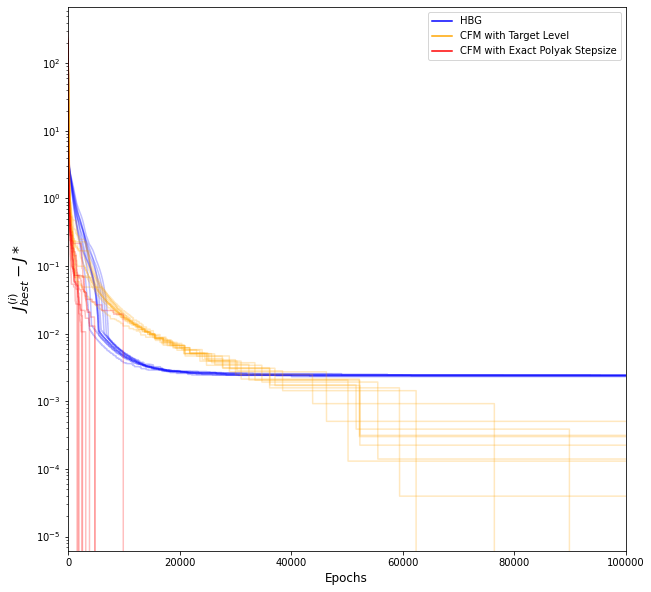
\includegraphics[width=.9\textwidth]{images/convex_100000.png}
        \caption{First 100.000 epochs}
        \label{fig:convex_100000}
    \end{subfigure}%
    \begin{subfigure}{.5\textwidth}
        \centering
        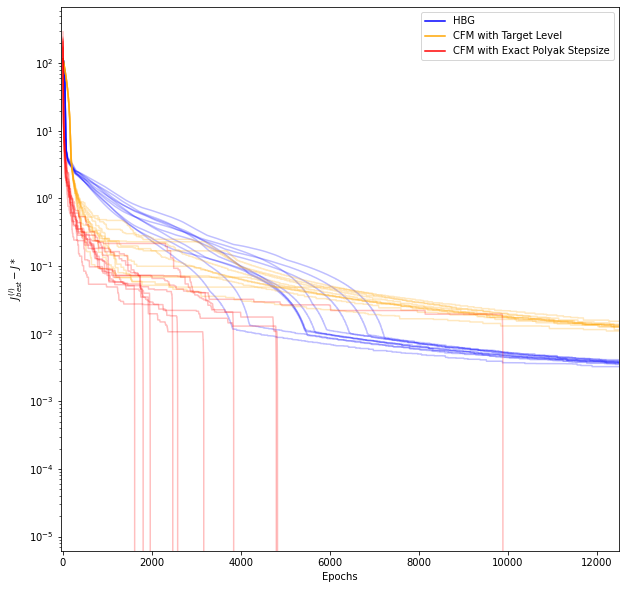
\includegraphics[width=.9\textwidth]{images/convex_12500.png}
        \caption{First 12.500 epochs}
        \label{fig:convex_12500}
    \end{subfigure}
    \caption{HBG, CFM with target level and CFM with exact Polyak step size convergence for a convex loss function}
    \label{fig:convex}
\end{figure}

As we can see, CFM with exact Polyak step size quickly outperforms the other two optimization algorithms, converging fast to our approximation of $J^*$ for every random run. CFM with target level, instead, takes much longer to converge; still, the convergence is steady, and we can appreciate the theoretical $\mathcal{O}(\epsilon^{-2})$ complexity. The same does not hold for HBG: even with a convex function, theoretical convergence is not guaranteed, as L-smoothness is further needed. As a matter of fact, HBG gets stuck in a suboptimal solution and gets slowly outperformed by CFM with target level. Still, it is noteworthy that HBG prevails over CFM from epoch $\sim$ 5.000 to epoch $\sim$ 35.000.

\subsection{Experiment 1 - MLP with one hidden layer}
\label{exp1}
In this experiment we considered two MLPs with one hidden layer consisting of 75 neurons, the first one with Sigmoid activation function and the second one with ReLU activation function. The Lasso regularization coeffienct was set to $\lambda = 0.01$ in both cases.

For both models we performed grid search as shown in table \ref{tab:1_gs}. As we observed some variance in training a model with CFM, we repeated each run of grid search for CFM for 5 times, each time with a different random weights initialization, and took their average as the result of the run. 

\begin{table}[htbp]
    \centering
    \begin{tabular}{|c|c|}
        \hline
        HBG & \makecell{$\alpha \in 10^{-3} \times \{0.5, 0.75, 1, 2.5, 5, 7.75, 10, 25, 50\}$ \\ $\beta \in \{0.1, 0.25, 0.5, 0.75, 0.9\}$} \\
        \hline
        CFM & \makecell{$\gamma \in \{0.5, 0.75, 1, 1.25, 1.5, 1.75\}$ \\ $a = 100$} \\
        \hline
    \end{tabular}
    \caption{Experiment 1 - Grid search set up}
    \label{tab:1_gs}
\end{table}

The results are shown in table \ref{tab:1_gsr} (CFM losses are the average ones, and we omit the variance as it always turned out to be negligible). We note that the best parameters combinations are the same both for Sigmoid and ReLU; still, ReLU allows a much better fitting of the training data, and achieves a much smaller loss. Once again, HBG seems to prefer high momentum, while the preferred step sizes are the medium ones. As for CFM, the best values of $\gamma$ oscillates much and the algorithm does not seem to have a particular tendency to favor low values of the hyperparameter over high values or vice versa.

\begin{table}[htbp]
    \begin{adjustwidth}{-2cm}{-2cm}
        \centering
        \begin{tabular}{|c c c|c c|c c c|c c|}
            \hline
            \multicolumn{5}{|c|}{Sigmoid} & \multicolumn{5}{c|}{ReLU} \\
            \hline
            \multicolumn{3}{|c|}{HBG} & \multicolumn{2}{c|}{CFM} & \multicolumn{3}{c|}{HBG} & \multicolumn{2}{c|}{CFM} \\
            \hline
            $\alpha$ & $\beta$ & loss & $\gamma$ & loss & $\alpha$ & $\beta$ & loss & $\gamma$ & loss \\
            \hline
            \textbf{0.025} & \textbf{0.9} & \textbf{1.188} & \textbf{0.75} & \textbf{1.200} & \textbf{0.025} & \textbf{0.9} & \textbf{0.864} & \textbf{0.75} & \textbf{0.889} \\
            0.05 & 0.9 & 1.190 & 1.25 & 1.233 & 0.05 & 0.5 & 0.866 & 1 & 0.894 \\
            0.05 & 0.75 & 1.236 & 1.75 & 1.245 & 0.05 & 0.75 & 0.867 & 0.5 & 0.898 \\
            \hline
        \end{tabular}
    \end{adjustwidth}
    \caption{Experiment 1 - Grid search results}
    \label{tab:1_gsr}
\end{table}

The best parameters combinations were then used to train the two models. The training was repeated for 25 times in both cases, each time with a different random weights initialization. The results are shown in table \ref{tab:1_r}; the convergence curves are shown in figure \ref{fig:h1}.

\begin{table}[htbp]
    \centering
    \begin{tabular}{|c|c|}
        \hline
        Sigmoid & \makecell{\textbf{HBG:} $\mathbf{1.210 \pm 0.020}$ \\ CFM: $1.407 \pm 0.661$} \\
        \hline
        ReLU & \makecell{\textbf{HBG:} $\mathbf{0.878 \pm 0.016}$ \\ CFM: $0.895 \pm 0.020$} \\
        \hline
    \end{tabular}
    \caption{Experiment 1 - Resulting losses}
    \label{tab:1_r}
\end{table}

\begin{figure}[htbp]
    \centering
    \begin{subfigure}{.5\textwidth}
        \centering
        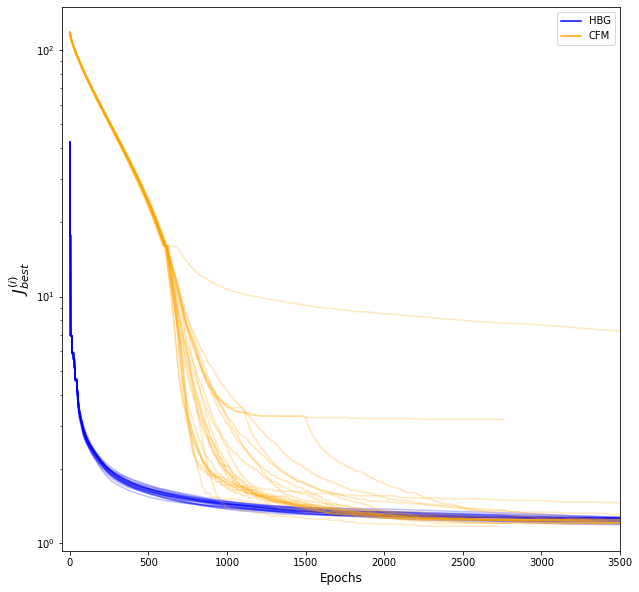
\includegraphics[width=.9\textwidth]{images/h1_sigmoid.png}
        \caption{Sigmoid}
        \label{fig:h1_sigmoid}
    \end{subfigure}%
    \begin{subfigure}{.5\textwidth}
        \centering
        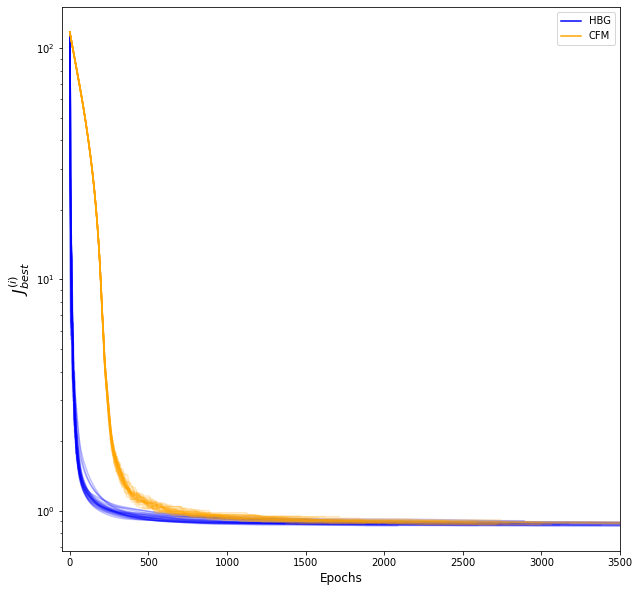
\includegraphics[width=.9\textwidth]{images/h1_relu.png}
        \caption{ReLU}
        \label{fig:h1_relu}
    \end{subfigure}
    \caption{HBG and CFM convergence for a one hidden layer MLP}
    \label{fig:h1}
\end{figure}

These results prove HBG superiority in both cases, in terms of accuracy and variance of the solution found. This is particularly evident in the case of Sigmoid activation function: CFM has a very high variance, and seems to easily get stuck into suboptimal solutions, while HBG rapidly and steadily converges. In the case of ReLU activation function, HBG superiority is much less evident, but still persistent.


\subsection{Experiment 2 - MLP with two hidden layers}
\label{exp2}
In this second experiment we increased the complexity of our models and built two MLPs, each one with two hidden layers, the first consisting of 60 neurons and the second of 30. We kept using Sigmoid activation function for the first MLP and ReLU for the second. Lasso regularization hyperparameter was set to $\lambda = 0.01$.

\begin{table}[htbp]
    \centering
    \begin{tabular}{|c|c|c|}
        \hline
        \multirow{2}{3.5em}{Sigmoid} & HBG & \makecell{$\alpha \in 10^{-3} \times \{0.5, 0.75, 1, 2.5, 5, 7.75, 10, 25, 50\}$ \\ $\beta \in \{0.1, 0.25, 0.5, 0.75, 0.9\}$} \\
        \cline{2-3}
         & CFM & \makecell{$\gamma \in \{0.5, 0.75, 1, 1.25, 1.5, 1.75, 1.9\}$ \\ $a = 150$} \\
        \hline
        \multirow{2}{3.5em}{ReLU} & HBG & \makecell{$\alpha \in 10^{-3} \times \{0.5, 0.75, 1, 2.5, 5, 7.75, 10, 25, 50\}$ \\ $\beta \in \{0.1, 0.25, 0.5, 0.75, 0.9\}$} \\
        \cline{2-3}
         & CFM & \makecell{$\gamma \in \{0.1, 0.15, 0.2, 0.3, 0.4, 0.5, 0.6, 0.75, 1, 1.25, 1.5\}$ \\ $a = 100$} \\
        \hline
    \end{tabular}
    \caption{Experiment 2 - Grid search set up}
    \label{tab:2_gs}
\end{table}

We fine tuned the hyperparameter by grid search, as shown in table \ref{tab:2_gs}. When performing grid search for CFM, we repeated each run for 5 times, and took their average as the result of the run.

The results are shown in table \ref{tab:2_gsr}. CFM losses in the case of ReLU are the average ones, and we omit the variance as it always turned out to be negligible. ReLU seems to allow a much better fitting of the training data, achieving a much smaller loss. HBG seems to prefer high momentum terms, with low step sizes for ReLU and medium step sizes for Sigmoid, while CFM seems not to have a particular tendency to favor low momentum over high momentum or vice versa. HBG seems superior in both cases, in particular with Sigmoid, where CFM loss is just too high and hugely variant.

\begin{table}[htpb]
    \begin{adjustwidth}{-2cm}{-2cm}
        \centering
        \begin{tabular}{|c c c|c c|c c c|c c|}
            \hline
            \multicolumn{5}{| c |}{Sigmoid} & \multicolumn{5}{ c |}{ReLU} \\
            \hline
            \multicolumn{3}{| c |}{HBG} & \multicolumn{2}{ c |}{CFM} & \multicolumn{3}{ c |}{HBG} & \multicolumn{2}{ c |}{CFM} \\
            \hline
            $\alpha$ & $\beta$ & loss & $\gamma$ & loss & $\alpha$ & $\beta$ & loss & $\gamma$ & loss \\
            \hline
            \textbf{0.05} & \textbf{0.9} & \textbf{1.401} & \textbf{0.75} & $\mathbf{5.267 \pm 5.540}$ & \textbf{0.00775} & \textbf{0.9} & \textbf{0.816} & \textbf{0.5} & \textbf{0.915} \\
            0.05 & 0.75 & 1.407 & 1.9 & $5.817 \pm 3.622$ & 0.01 & 0.9 & 0.818 & 0.6 & 1.005 \\
            0.025 & 0.9 & 1.444 & 1.5 & $7.084 \pm 4.911$ & 0.005 & 0.9 & 0.830 & 0.15 & 1.075 \\
            \hline
        \end{tabular}
    \end{adjustwidth}
    \caption{Experiment 2 - Grid search results}
    \label{tab:2_gsr}
\end{table}

The best parameters combination were used to train the two models. We repeated the training for 25 times, each time with a different random weights initialization. The results are shown in table \ref{tab:2_r}; the convergence curves are shown in figure \ref{fig:h2}.

\begin{figure}[htbp]
    \centering
    \begin{subfigure}{.5\textwidth}
        \centering
        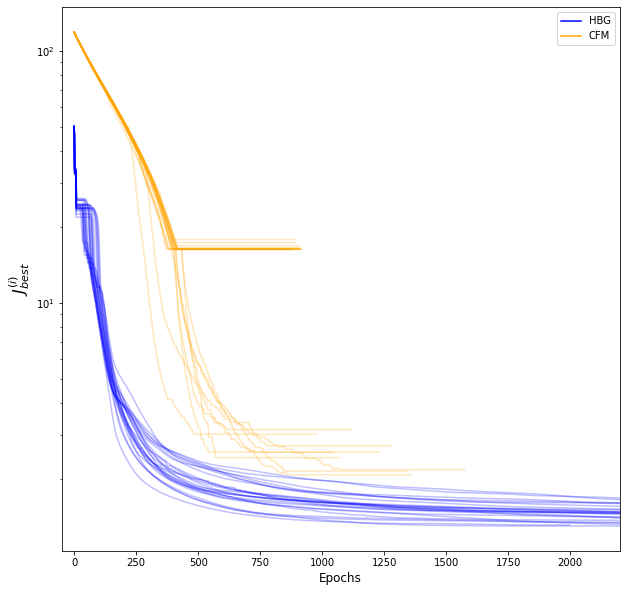
\includegraphics[width=.9\textwidth]{images/h2_sigmoid.png}
        \caption{Sigmoid}
        \label{fig:h2_sigmoid}
    \end{subfigure}%
    \begin{subfigure}{.5\textwidth}
        \centering
        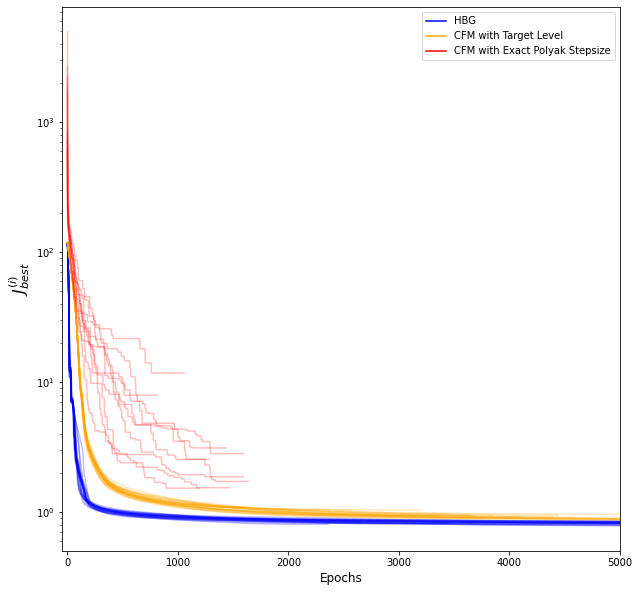
\includegraphics[width=.9\textwidth]{images/h2_relu.png}
        \caption{ReLU}
        \label{fig:h2_relu}
    \end{subfigure}
    \caption{HBG and CFM convergence for a two hidden layers MLP}
    \label{fig:h2}
\end{figure}

As we can see, HBG outperforms CFM in both cases, both in terms of optimality of the solution and in terms of variance, with a steady and faster convergence. CFM convergence compares decently to that of HBG in the case of ReLU, while in the case of Sigmoid is very chaotic, and gets stuck into multiple suboptimal solutions.

\begin{table}[htbp]
    \centering
    \begin{tabular}{|c|c|}
        \hline
        Sigmoid & \makecell{\textbf{HBG:} $\mathbf{1.353 \pm 0.045}$ \\ CFM: $11.502 \pm 6.734$} \\
        \hline
        ReLU & \makecell{\textbf{HBG:} $\mathbf{0.816 \pm 0.017}$ \\ CFM: $0.942 \pm 0.068$} \\
        \hline
    \end{tabular}
    \caption{Experiment 2 - Resulting Losses}
    \label{tab:2_r}
\end{table}

The results we got for CFM in the case of Sigmoid were so bad that we repeated the whole process with different values of $a$. We omit the intermediate results and just show the convergence curves in figure \ref{fig:h2_sigmoid_a}. We note that lower values of $a$ allow for some of the runs to achieve better losses, while larger values speed up the convergence, as we could have expected (cfr. \ref{exp01}). Still, the overall quality of the convergence does not seem to improve, and the variance remains very high and independent of the value of $a$.

\begin{figure}[htbp]
    \centering
    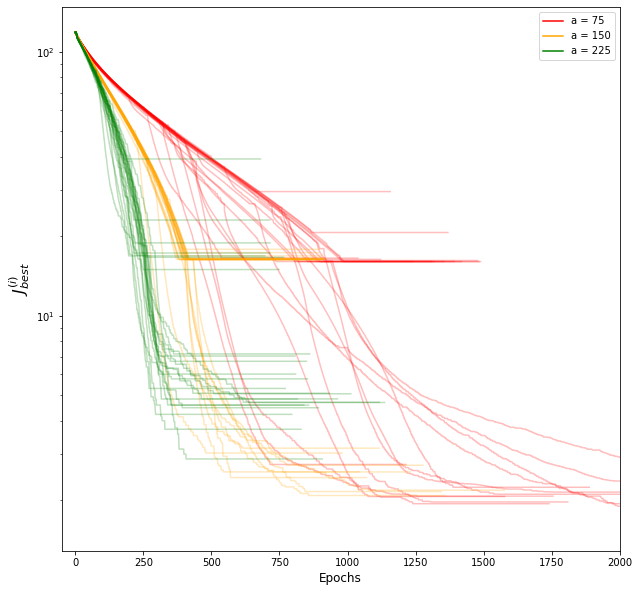
\includegraphics[width=.6\textwidth]{images/h2_sigmoid_a.png}
    \caption{CFM convergence for a two hidden layers MLP for $a=75,150,225$}
    \label{fig:h2_sigmoid_a}
\end{figure}

As a further step, we wanted to test CFM with exact Polyak step size in the case of ReLU. Thus, we used the value 0.816 from table \ref{tab:2_r} to approximate $J^*$, and fine tuned the momentum hyperparameter by grid search, choosing the best $\gamma \in \{0.1, 0.15, 0.2, 0.3, 0.4, 0.5, 0.6, 0.75, 1, 1.25, 1.5\}$. We kept the usage of 5 random initializations for each grid search run, but we increased the early stopping patience to 500 epochs. The results are shown in table \ref{tab:2_bl_r}. The algorithm prefers low momentum, but does not seem capable of getting close to the results achieved by CFM with target level and HBG.

\begin{table}[htbp]
    \centering
    \begin{tabular}{|c c|}
        \hline
        $\gamma$ & loss \\
        \hline
        \textbf{0.2} & $\mathbf{3.486 \pm 2.572}$ \\
        0.15 & $4.284 \pm 2.987$ \\
        0.1 & $4.523 \pm 2.207$ \\
        \hline
    \end{tabular}
    \caption{Experiment 2 - Grid search results for CFM with exact Polyak step size.}
    \label{tab:2_bl_r}
\end{table}

The best value of $\gamma$ was then used to train the model for 10 times, each time with a different random weights initialization, achieving a final loss of $3.762 \pm 3.207$ (the convergence curves are also shown in figure \ref{fig:h2}), a result not even remotely comparable to those obtained by CFM with target level and HBG.

\subsection{Experiment 3 - MLP with three hidden layers}
\label{exp3}
In this last experiment we increased even more the complexity of our model and built a MLP with three hidden layers, with respectively 60, 45 and 30 neurons, but we limited ourselves to consider only the ReLU as activation function. We also increased the value of Lasso regularization hyperparameter to $\lambda =0.1$.
First, we fine tuned CFM and HBG hyperparameters by grid search, as shown in table \ref{tab:3_gs}. As usual, we repeated each run of grid search for CFM 5 times, and took their average as the result of the run, to better deal with the high variance of the algorithm.

\begin{table}[htbp]
    \centering
    \begin{tabular}{|c|c|}
        \hline
        HBG & \makecell{$\alpha \in 10^{-3} \times \{0.5, 0.75, 1, 2.5, 5, 7.75, 10, 25, 50\}$ \\ $\beta \in \{0.1, 0.25, 0.5, 0.75, 0.9\}$} \\
        \hline
         CFM & \makecell{$\gamma \in \{0.3, 0.4, 0.5, 0.6, 0.75, 1, 1.25\}$ \\ $a = 100$} \\
        \hline
    \end{tabular}
    \caption{Experiment 3 - Grid search set up}
    \label{tab:3_gs}
\end{table}

The results are shown in table \ref{tab:3_gsr}. HBG seems to prefer medium-low step sizes and very high momentum, while CFM tends to favor medium-low momentum terms. CFM also seems to have a quite high variance, but is able to achieve far better results.

\begin{table}[htbp]
    \centering
    \begin{tabular}{|c c c | c c|}
        \hline
        \multicolumn{3}{| c |}{HBG} & \multicolumn{2}{ c |}{CFM} \\
        \hline
        $\alpha$ & $\beta$ & loss & $\gamma$ & loss \\
        \hline
        \textbf{0.001} & \textbf{0.9} & \textbf{15.867} & \textbf{0.6} & $\mathbf{4.815 \pm 0.739}$ \\
        0.0025 & 0.9 & 15.882 & 0.4 & $4.959 \pm 2.666$ \\
        0.00075 & 0.9 & 15.887 & 0.3 & $6.139 \pm 5.424$ \\
        \hline
    \end{tabular}
    \caption{Experiment 3 - Grid search results}
    \label{tab:3_gsr}
\end{table}

We used the best combinations of parameters found by grid search to train the model. We repeated the training for 25 times, each time with random initialization. At the end, CFM was able to achieve a loss of $5.549 \pm 2.414$, while HBG could not improve over $15.881 \pm 0.010$. The convergence curves are shown in figure \ref{fig:h3_relu}.

\begin{figure}[htbp]
    \centering
    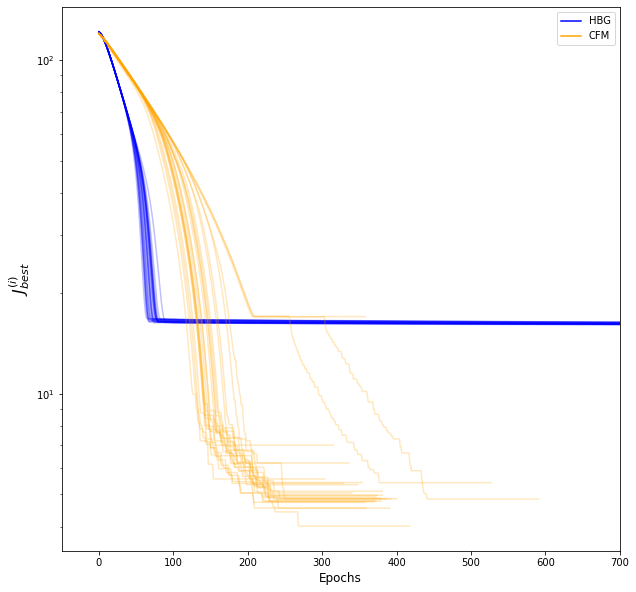
\includegraphics[width=.6\textwidth]{images/h3_relu.png}
    \caption{HBG and CFM convergence for a three hidden layers MLP}
    \label{fig:h3_relu}
\end{figure}

As we can see, even if with a much higher variance, CFM is able to achieve far better solutions, while HBG can't avoid getting stuck into a local minimum, and is easily outperformed by CFM.